\documentclass{extbook}[14pt]
\usepackage{multicol, enumerate, enumitem, hyperref, color, soul, setspace, parskip, fancyhdr, amssymb, amsthm, amsmath, latexsym, units, mathtools}
\everymath{\displaystyle}
\usepackage[headsep=0.5cm,headheight=0cm, left=1 in,right= 1 in,top= 1 in,bottom= 1 in]{geometry}
\usepackage{dashrule}  % Package to use the command below to create lines between items
\newcommand{\litem}[1]{\item #1

\rule{\textwidth}{0.4pt}}
\pagestyle{fancy}
\lhead{}
\chead{Answer Key for Progress Quiz 7 Version B}
\rhead{}
\lfoot{4173-5738}
\cfoot{}
\rfoot{Spring 2021}
\begin{document}
\textbf{This key should allow you to understand why you choose the option you did (beyond just getting a question right or wrong). \href{https://xronos.clas.ufl.edu/mac1105spring2020/courseDescriptionAndMisc/Exams/LearningFromResults}{More instructions on how to use this key can be found here}.}

\textbf{If you have a suggestion to make the keys better, \href{https://forms.gle/CZkbZmPbC9XALEE88}{please fill out the short survey here}.}

\textit{Note: This key is auto-generated and may contain issues and/or errors. The keys are reviewed after each exam to ensure grading is done accurately. If there are issues (like duplicate options), they are noted in the offline gradebook. The keys are a work-in-progress to give students as many resources to improve as possible.}

\rule{\textwidth}{0.4pt}

\begin{enumerate}\litem{
Construct the lowest-degree polynomial given the zeros below. Then, choose the intervals that contain the coefficients of the polynomial in the form $ax^3+bx^2+cx+d$.
\[ -6, \frac{7}{2}, \text{ and } -7 \]The solution is \( 2x^{3} +19 x^{2} -7 x -294 \), which is option B.\begin{enumerate}[label=\Alph*.]
\item \( a \in [1, 3], b \in [4, 18], c \in [-85, -74], \text{ and } d \in [-296, -290] \)

$2x^{3} +9 x^{2} -77 x -294$, which corresponds to multiplying out $(x -6)(2x + 7)(x + 7)$.
\item \( a \in [1, 3], b \in [19, 24], c \in [-10, -5], \text{ and } d \in [-296, -290] \)

* $2x^{3} +19 x^{2} -7 x -294$, which is the correct option.
\item \( a \in [1, 3], b \in [-21, -18], c \in [-10, -5], \text{ and } d \in [290, 297] \)

$2x^{3} -19 x^{2} -7 x + 294$, which corresponds to multiplying out $(x -6)(2x + 7)(x -7)$.
\item \( a \in [1, 3], b \in [19, 24], c \in [-10, -5], \text{ and } d \in [290, 297] \)

$2x^{3} +19 x^{2} -7 x + 294$, which corresponds to multiplying everything correctly except the constant term.
\item \( a \in [1, 3], b \in [-9, -4], c \in [-96, -85], \text{ and } d \in [290, 297] \)

$2x^{3} -5 x^{2} -91 x + 294$, which corresponds to multiplying out $(x -6)(2x -7)(x + 7)$.
\end{enumerate}

\textbf{General Comment:} To construct the lowest-degree polynomial, you want to multiply out $(x + 6)(2x -7)(x + 7)$
}
\litem{
Which of the following equations \textit{could} be of the graph presented below?

\begin{center}
    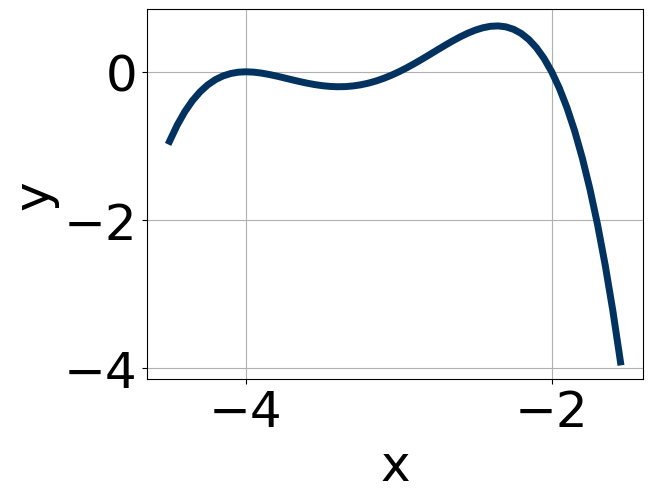
\includegraphics[width=0.5\textwidth]{../Figures/polyGraphToFunctionB.png}
\end{center}


The solution is \( -3(x + 4)^{4} (x + 2)^{5} (x + 3)^{5} \), which is option A.\begin{enumerate}[label=\Alph*.]
\item \( -3(x + 4)^{4} (x + 2)^{5} (x + 3)^{5} \)

* This is the correct option.
\item \( -7(x + 4)^{9} (x + 2)^{10} (x + 3)^{5} \)

The factor $-4$ should have an even power and the factor $-2$ should have an odd power.
\item \( 10(x + 4)^{6} (x + 2)^{5} (x + 3)^{6} \)

The factor $(x + 3)$ should have an odd power and the leading coefficient should be the opposite sign.
\item \( -4(x + 4)^{4} (x + 2)^{4} (x + 3)^{11} \)

The factor $(x + 2)$ should have an odd power.
\item \( 18(x + 4)^{4} (x + 2)^{7} (x + 3)^{5} \)

This corresponds to the leading coefficient being the opposite value than it should be.
\end{enumerate}

\textbf{General Comment:} General Comments: Draw the x-axis to determine which zeros are touching (and so have even multiplicity) or cross (and have odd multiplicity).
}
\litem{
Describe the zero behavior of the zero $x = -4$ of the polynomial below.
\[ f(x) = 7(x - 8)^{5}(x + 8)^{2}(x + 4)^{10}(x - 4)^{5} \]The solution is the graph below, which is option C.
\begin{center}
    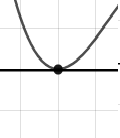
\includegraphics[width=0.3\textwidth]{../Figures/polyZeroBehaviorCB.png}
\end{center}\begin{enumerate}[label=\Alph*.]
\begin{multicols}{2}
\item 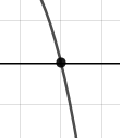
\includegraphics[width = 0.3\textwidth]{../Figures/polyZeroBehaviorAB.png}
\item 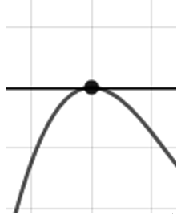
\includegraphics[width = 0.3\textwidth]{../Figures/polyZeroBehaviorBB.png}
\item 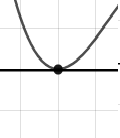
\includegraphics[width = 0.3\textwidth]{../Figures/polyZeroBehaviorCB.png}
\item 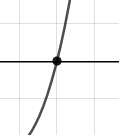
\includegraphics[width = 0.3\textwidth]{../Figures/polyZeroBehaviorDB.png}
\end{multicols}\item None of the above.\end{enumerate}
\textbf{General Comment:} You will need to sketch the entire graph, then zoom in on the zero the question asks about.
}
\litem{
Construct the lowest-degree polynomial given the zeros below. Then, choose the intervals that contain the coefficients of the polynomial in the form $x^3+bx^2+cx+d$.
\[ 4 - 4 i \text{ and } 4 \]The solution is \( x^{3} -12 x^{2} +64 x -128 \), which is option A.\begin{enumerate}[label=\Alph*.]
\item \( b \in [-15, -11], c \in [61, 66], \text{ and } d \in [-132, -126] \)

* $x^{3} -12 x^{2} +64 x -128$, which is the correct option.
\item \( b \in [4, 17], c \in [61, 66], \text{ and } d \in [124, 131] \)

$x^{3} +12 x^{2} +64 x + 128$, which corresponds to multiplying out $(x-(4 - 4 i))(x-(4 + 4 i))(x + 4)$.
\item \( b \in [-3, 6], c \in [-4, 2], \text{ and } d \in [-19, -15] \)

$x^{3} + x^{2} -16$, which corresponds to multiplying out $(x + 4)(x -4)$.
\item \( b \in [-3, 6], c \in [-8, -5], \text{ and } d \in [16, 20] \)

$x^{3} + x^{2} -8 x + 16$, which corresponds to multiplying out $(x -4)(x -4)$.
\item \( \text{None of the above.} \)

This corresponds to making an unanticipated error or not understanding how to use nonreal complex numbers to create the lowest-degree polynomial. If you chose this and are not sure what you did wrong, please contact the coordinator for help.
\end{enumerate}

\textbf{General Comment:} Remember that the conjugate of $a+bi$ is $a-bi$. Since these zeros always come in pairs, we need to multiply out $(x-(4 - 4 i))(x-(4 + 4 i))(x-(4))$.
}
\litem{
Construct the lowest-degree polynomial given the zeros below. Then, choose the intervals that contain the coefficients of the polynomial in the form $ax^3+bx^2+cx+d$.
\[ -2, \frac{-3}{5}, \text{ and } \frac{1}{3} \]The solution is \( 15x^{3} +34 x^{2} +5 x -6 \), which is option D.\begin{enumerate}[label=\Alph*.]
\item \( a \in [9, 26], b \in [-32, -20], c \in [-11, -8], \text{ and } d \in [2, 11] \)

$15x^{3} -26 x^{2} -11 x + 6$, which corresponds to multiplying out $(x -2)(5x + 3)(3x -1)$.
\item \( a \in [9, 26], b \in [31, 43], c \in [0, 11], \text{ and } d \in [2, 11] \)

$15x^{3} +34 x^{2} +5 x + 6$, which corresponds to multiplying everything correctly except the constant term.
\item \( a \in [9, 26], b \in [-48, -38], c \in [29, 33], \text{ and } d \in [-6, -3] \)

$15x^{3} -44 x^{2} +31 x -6$, which corresponds to multiplying out $(x -2)(5x -3)(3x -1)$.
\item \( a \in [9, 26], b \in [31, 43], c \in [0, 11], \text{ and } d \in [-6, -3] \)

* $15x^{3} +34 x^{2} +5 x -6$, which is the correct option.
\item \( a \in [9, 26], b \in [-34, -33], c \in [0, 11], \text{ and } d \in [2, 11] \)

$15x^{3} -34 x^{2} +5 x + 6$, which corresponds to multiplying out $(x -2)(5x -3)(3x + 1)$.
\end{enumerate}

\textbf{General Comment:} To construct the lowest-degree polynomial, you want to multiply out $(x + 2)(5x + 3)(3x -1)$
}
\litem{
Describe the zero behavior of the zero $x = 5$ of the polynomial below.
\[ f(x) = 4(x - 5)^{2}(x + 5)^{5}(x + 8)^{6}(x - 8)^{9} \]The solution is the graph below, which is option B.
\begin{center}
    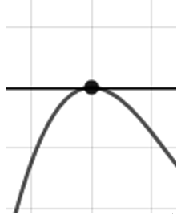
\includegraphics[width=0.3\textwidth]{../Figures/polyZeroBehaviorCopyBB.png}
\end{center}\begin{enumerate}[label=\Alph*.]
\begin{multicols}{2}
\item 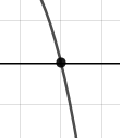
\includegraphics[width = 0.3\textwidth]{../Figures/polyZeroBehaviorCopyAB.png}
\item 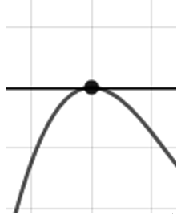
\includegraphics[width = 0.3\textwidth]{../Figures/polyZeroBehaviorCopyBB.png}
\item 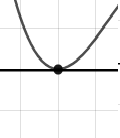
\includegraphics[width = 0.3\textwidth]{../Figures/polyZeroBehaviorCopyCB.png}
\item 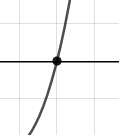
\includegraphics[width = 0.3\textwidth]{../Figures/polyZeroBehaviorCopyDB.png}
\end{multicols}\item None of the above.\end{enumerate}
\textbf{General Comment:} You will need to sketch the entire graph, then zoom in on the zero the question asks about.
}
\litem{
Describe the end behavior of the polynomial below.
\[ f(x) = -7(x + 8)^{4}(x - 8)^{9}(x + 6)^{5}(x - 6)^{5} \]The solution is the graph below, which is option A.
\begin{center}
    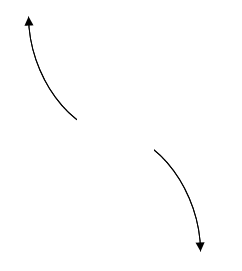
\includegraphics[width=0.3\textwidth]{../Figures/polyEndBehaviorCopyAB.png}
\end{center}\begin{enumerate}[label=\Alph*.]
\begin{multicols}{2}
\item 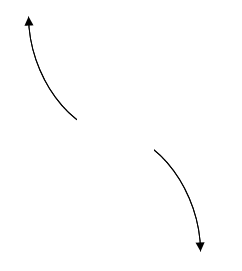
\includegraphics[width = 0.3\textwidth]{../Figures/polyEndBehaviorCopyAB.png}
\item 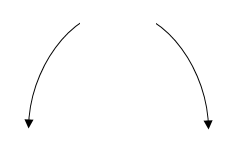
\includegraphics[width = 0.3\textwidth]{../Figures/polyEndBehaviorCopyBB.png}
\item 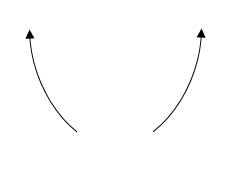
\includegraphics[width = 0.3\textwidth]{../Figures/polyEndBehaviorCopyCB.png}
\item 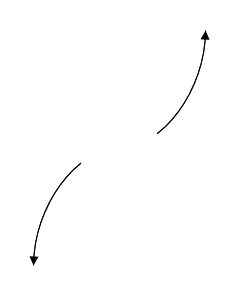
\includegraphics[width = 0.3\textwidth]{../Figures/polyEndBehaviorCopyDB.png}
\end{multicols}\item None of the above.\end{enumerate}
\textbf{General Comment:} Remember that end behavior is determined by the leading coefficient AND whether the \textbf{sum} of the multiplicities is positive or negative.
}
\litem{
Describe the end behavior of the polynomial below.
\[ f(x) = 6(x + 9)^{4}(x - 9)^{9}(x + 5)^{5}(x - 5)^{7} \]The solution is the graph below, which is option D.
\begin{center}
    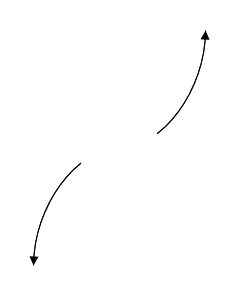
\includegraphics[width=0.3\textwidth]{../Figures/polyEndBehaviorDB.png}
\end{center}\begin{enumerate}[label=\Alph*.]
\begin{multicols}{2}
\item 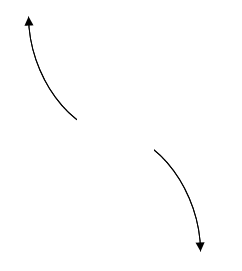
\includegraphics[width = 0.3\textwidth]{../Figures/polyEndBehaviorAB.png}
\item 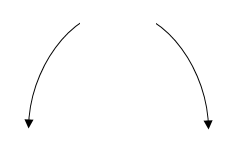
\includegraphics[width = 0.3\textwidth]{../Figures/polyEndBehaviorBB.png}
\item 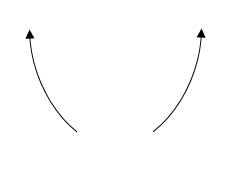
\includegraphics[width = 0.3\textwidth]{../Figures/polyEndBehaviorCB.png}
\item 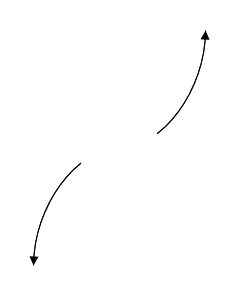
\includegraphics[width = 0.3\textwidth]{../Figures/polyEndBehaviorDB.png}
\end{multicols}\item None of the above.\end{enumerate}
\textbf{General Comment:} Remember that end behavior is determined by the leading coefficient AND whether the \textbf{sum} of the multiplicities is positive or negative.
}
\litem{
Which of the following equations \textit{could} be of the graph presented below?

\begin{center}
    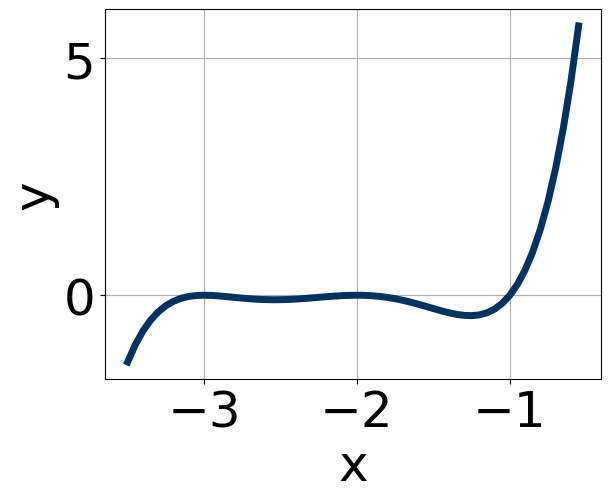
\includegraphics[width=0.5\textwidth]{../Figures/polyGraphToFunctionCopyB.png}
\end{center}


The solution is \( 20(x + 3)^{6} (x + 2)^{6} (x + 1)^{5} \), which is option A.\begin{enumerate}[label=\Alph*.]
\item \( 20(x + 3)^{6} (x + 2)^{6} (x + 1)^{5} \)

* This is the correct option.
\item \( 11(x + 3)^{8} (x + 2)^{5} (x + 1)^{7} \)

The factor $(x + 2)$ should have an even power.
\item \( -11(x + 3)^{6} (x + 2)^{6} (x + 1)^{7} \)

This corresponds to the leading coefficient being the opposite value than it should be.
\item \( 18(x + 3)^{8} (x + 2)^{7} (x + 1)^{10} \)

The factor $(x + 2)$ should have an even power and the factor $(x + 1)$ should have an odd power.
\item \( -14(x + 3)^{8} (x + 2)^{4} (x + 1)^{10} \)

The factor $(x + 1)$ should have an odd power and the leading coefficient should be the opposite sign.
\end{enumerate}

\textbf{General Comment:} General Comments: Draw the x-axis to determine which zeros are touching (and so have even multiplicity) or cross (and have odd multiplicity).
}
\litem{
Construct the lowest-degree polynomial given the zeros below. Then, choose the intervals that contain the coefficients of the polynomial in the form $x^3+bx^2+cx+d$.
\[ 5 - 5 i \text{ and } 3 \]The solution is \( x^{3} -13 x^{2} +80 x -150 \), which is option A.\begin{enumerate}[label=\Alph*.]
\item \( b \in [-16, -9], c \in [79, 86], \text{ and } d \in [-157, -147] \)

* $x^{3} -13 x^{2} +80 x -150$, which is the correct option.
\item \( b \in [-8, 10], c \in [2, 7], \text{ and } d \in [-19, -11] \)

$x^{3} + x^{2} +2 x -15$, which corresponds to multiplying out $(x + 5)(x -3)$.
\item \( b \in [10, 14], c \in [79, 86], \text{ and } d \in [149, 151] \)

$x^{3} +13 x^{2} +80 x + 150$, which corresponds to multiplying out $(x-(5 - 5 i))(x-(5 + 5 i))(x + 3)$.
\item \( b \in [-8, 10], c \in [-9, -2], \text{ and } d \in [12, 16] \)

$x^{3} + x^{2} -8 x + 15$, which corresponds to multiplying out $(x -5)(x -3)$.
\item \( \text{None of the above.} \)

This corresponds to making an unanticipated error or not understanding how to use nonreal complex numbers to create the lowest-degree polynomial. If you chose this and are not sure what you did wrong, please contact the coordinator for help.
\end{enumerate}

\textbf{General Comment:} Remember that the conjugate of $a+bi$ is $a-bi$. Since these zeros always come in pairs, we need to multiply out $(x-(5 - 5 i))(x-(5 + 5 i))(x-(3))$.
}
\end{enumerate}

\end{document}